\question Lee con atención a cada problema y responde a las preguntas de cada uno.

% \begin{multicols}{2}
\begin{parts}
    \setlength{\columnsep}{30pt}
    \begin{multicols}{2}
        \part[5] Matisyahu tomó una porción de pizza del congelador y la puso en el horno.
        Se graficó la temperatura de la pizza (en grados Celsius) como una función del tiempo (en minutos), en la Figura \ref{fig:pizza_temp}.

        \begin{figure}[H]
            \centering
            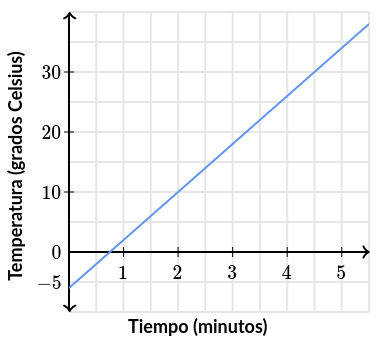
\includegraphics[width=0.7\linewidth]{../images/pizza_temp}
            \label{fig:pizza_temp}
        \end{figure}
        \textbf{¿Qué tan rápido calentó el horno la pizza?}

        \begin{oneparchoices}
            \choice 0.80 $^\circ$C/min
            \choice 10 $^\circ$C/min\\
            \choice 0.9  $^\circ$C/min
            \CorrectChoice 8 $^\circ$C/min
        \end{oneparchoices}

        \part[5] Karl viajó a Alaska en su camión.
        Se graficó la cantidad de combustible que queda en el tanque del camión (en litros) como una función de la distancia que recorrió (en kilómetros), en la Figura \ref{fig:alaska_combustible}.

        \begin{figure}[H]
            \centering
            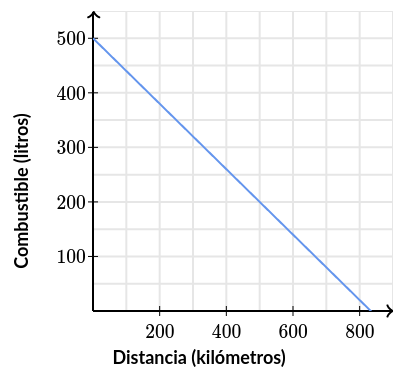
\includegraphics[width=0.7\linewidth]{../images/alaska_combustible}
            \label{fig:alaska_combustible}
        \end{figure}

        \textbf{¿Cuánto combustible consume el tanque cada 100 kilómetros?}

        \begin{oneparchoices}
            \choice 60 L
            \choice 0.5 L
            \choice 500 L
            \choice 0.6 L
        \end{oneparchoices}
    \end{multicols}
    \begin{multicols}{2}
        \part[5] A Scott le gusta correr distancias largas. Puede correr
        20 km en 85 minutos. Él quiere saber cuántos minutos le tomará correr 52 km al mismo paso.

        \textbf{¿Cuánto tardará Scott en correr 52 km?}

        \fillin[221][1cm] minutos.

        \part[5] Teresa está cuidando una fogata. Ha mantenido el fuego
        ardiendo durante 4 horas con 6 troncos. Ella quiere saber cuántos
        troncos necesita para
        mantener el fuego ardiendo durante 18 horas. Para sus cálculos,
        ella supone que todos los troncos son iguales.

        \textbf{¿Cuántos troncos necesita Teresa para mantener el fuego durante 18 horas?}

        \fillin[27][1cm] troncos.

        \part[5] A Ted le gusta correr distancias largas. Puede correr
        20 km en 95 minutos. Él quiere saber cuántos kilómetros (k) recorrerá si corre al mismo paso durante 285 minutos.


        \textbf{¿Cuánto correrá Ted en 285 minutos?}

        \fillin[60][1cm] kilómetros.

        \part[5] El agente Hunt transfiere archivos clasificados del computador principal de la CIA a su unidad USB.
        La variable $S$ modela el tamaño de los archivos (en megabytes) en la unidad después de $t$ segundos de transferencia.

        \[S=5t+45\]

        \textbf{¿Cuántos megabytes transfiere el agente Hunt cada 10 segundos?}

        \fillin[50][1cm] megabytes.

        \columnbreak

        \part[5] Harry obtuvo un préstamo del banco.
        La variable $D$ modela la deuda restante de Harry (en pesos) como función del tiempo $t$ en meses desde que obtuvo el préstamo.

        \[D=-200t+9000\]

        \textbf{¿Cuánto dinero paga Harry cada mes?}

        \$\fillin[200][1cm]

        \part[5] Andrei quiere llenar un tanque de vidrio con canicas, y luego el espacio restante con agua.
        La variable $w$ modela la cantidad de agua (en litros) que Andrei usa si utiliza $n$ canicas.

        \[w=32-0.05n\]

        \textbf{¿Cuál es el volumen de cada canica?}

        \fillin[0.05][1cm] litros.

        \part[5] La temperatura puede medirse en dos unidades comunes: grados Celsius y grados Fahrenheit.
        La variable $F$ representa la temperatura en grados Fahrenheit que es equivalente a la temperatura $C$ en grados Celsius.

        \[F=32+1.8C\]

        \textbf{¿Cuál es el incremento en grados Fahrenheit equivalente a un incremento de 10 grados Celsius?}

        \fillin[0.05][1cm] grados Fahrenheit.

    \end{multicols}
\end{parts}
% \end{multicols}
